\documentclass{article} % Packages für die unterstüztung der deutschen Sprache
\usepackage{ucs}
\usepackage[utf8x]{inputenc}
\usepackage[T1]{fontenc}
\usepackage[ngerman]{babel}
\usepackage{blindtext}
\usepackage{multicol}
\usepackage{titlesec}
\usepackage{wrapfig}
\usepackage[a4paper, margin=4mm]{geometry}

% Package für das einfügen von Bildern
\usepackage{graphicx}

\newenvironment{floatfig}
  {\par\medskip\noindent\minipage{\linewidth}}
  {\endminipage\par\medskip}

\title{BEBU Spicker MAP 2017}
\author{Yanik Künzi}
\date{\today{}, Lyss}

\begin{document}
	\begin{minipage}[t][0.8\textheight]{0.97\textwidth}
	 \begin{multicols*}{4}
		\begin{flushleft}
		{\tiny
			\noindent Bei der \textbf{Aussenfinanzierung} werden finanzielle 
			Mittel aus unternehmensexternen Quellen zugeführt.
			D.h., es fließt Geld von außen
			in das Unternehmen, welches nicht aus den
			Umsätzen des Unternehmens stammt.
			Beispiele für Außenfinanzierung sind die Ausgabe
			von \textit{z.B. Aktien (Beteiligungsfinanzierung),
			Bankdarlehen oder Lieferantenkredite.}
			\noindent\rule{\linewidth}{0.4pt}
			\textbf{Kartelle} im Bereich der Wirtschaft ist ein
			Vertrag oder Beschluss zwischen selbständig
			bleibenden Unternehmen oder sonstigen
			Marktakteuren der gleichen Marktseite zur
			Beschränkung ihres Wettbewerbs. Kartelle sind
			Vereinbarungen oder auf andere Weise
			abgesprochene Kooperationen von rechtlich
			selbstständigen Unternehmungen zur
			Beschränkung des Wettbewerbs.
			\noindent\rule{\linewidth}{0.4pt}
			Die \textbf{Kontrollspanne} (Führungsspanne) ist
			die Anzahl Mitarbeiter, die einer
			Führungskraft (Linienstelle) direkt unterstellt
			sind. Dazu zählen sowohl Linien- als auch Stabstellen.
			\noindent\rule{\linewidth}{0.4pt}
			\textbf{Fusion} : Verschmelzung bisher selbständiger
			Unternehmen zu einem rechtlich und
			wirtschaftlich einheitlichen Unternehmen. Es
			entsteht eine neue Firma (A + B = C)!
			\textbf{Übernahme} : Bei einer Übernahme wird eine
			Firma komplett übernommen. (B gehört neu zu A)
			\textbf{Joint-Venture} : spezifische Kooperationsform;
			die Partnerunternehmen sind jeweils mit Kapital
			am Joint Venture beteiligt, tragen gemeinsam das
			finanzielle Risiko der Investition und nehmen
			Führungsfunktionen
			im gemeinsamen Unternehmen wahr. (A + B
			gründen gemeinsam C = C ist ein Joint Venture)
			\noindent\rule{\linewidth}{0.4pt}
			Unter \textbf{Steuerprogression} versteht man das
			Ansteigen des Steuersatzes in Abhängigkeit vom
			zu versteuernden Einkommen oder Vermögen.
			(Kurve wird immer steiler / exponential).
			\textbf{Kalte Progression} ist die
			Steuermehrbelastung, die dann eintritt, wenn die
			Einkommensteuersätze nicht der
			Preissteigerung angepasst werden.
			\textit{Beispiel: habe 60'000.- das hat eine Kaufkraft,
			nach einem Jahr Teuerung, nicht mehr dieselbe
			Kaufkraft.Es gibt eine Lohnerhöhung, habe dann
			65'000, wieder Teuerung, wieder Lohnerhöhung
			dann 70'000, kann dann immer noch das selbe
			kaufen. Trotz selber Kaufkraft mehr Steuern. Ist
			dann eine kalte Progression. Höhere Steuern
			durch nicht beachten der Teuerung seitens
			Steuern.}
			\noindent\rule{\linewidth}{0.4pt}
			\textbf{Statuten} sind sowohl für Aktiengesellschaften
			als auch für Gesellschaften mit beschränkter
			Haftung (GmbH) gesetzlich vorgeschrieben.
			Statuten müssen notariell beglaubigt sein.
			Statuten variieren je nach Rechtsform. Sie sind
			Gesetzmässigkeiten für eine Rechtsform.
			Folgende Angaben gehören in die Statuten:
			\begin{itemize}
				\item Firma, Sitz und Zweck der Gesellschaft
				\item Höhe des Stammkapitals
			\end{itemize}
			\noindent\rule{\linewidth}{0.4pt}
			\textbf{Risikokapital} - auch Venture-Capital oder
			Wagniskapital genannt – ist außerbörsliches
			Beteiligungskapital („private equity“), das eine
			Beteiligungsgesellschaft (Venture-Capital-
			Gesellschaft) zur Beteiligung an als besonders
			riskant geltenden Unternehmungen bereitstellt.
			\underline{Eigenkapital ist} \par\noindent\underline{Risikokapital.}
			\newline\noindent\rule{\linewidth}{0.4pt}
			Ein Unternehmen weist im Bereich \textbf{Anlagen}
			Investitionsgüter \textbf{(Anlagevermögen)} aus.
			\textbf{Konsumgüter} werden im \textbf{Umlaufvermögen} im
			Bereich Vorräte verbucht.
			\noindent\rule{\linewidth}{0.4pt}
			Die drei \textbf{Wirtschaftssektoren} sind der primäre
			(Ressourcengewinnung), der sekundäre (Industrie)
			und der tertiäre (Dienstleistungen).
			Beispiel: PC-Herstellung: 2, Software: 3,
			Treuhänder: 3, Fleisch (Bauer / Metzger /
			Migros): 1/2/3
			\noindent\rule{\linewidth}{0.4pt}
			\textbf{Sortiment} - 
			Tiefes Sortiment: weniger Produktgruppen, aber
			sehr grosse Auswahl dieser
			Breites Sortiment: viele verschiedene
			Produktgruppen
			\noindent\rule{\linewidth}{0.4pt}
			\textbf{Vorteile des Zwischenhandels für die Kunden}
			\begin{itemize}
				\item Standortfunktion (Kundennähe)
				\item Sortimentsfunktion (Produkte von mehreren
				Herstellern)
				\item Lagerfunktion (auch Maklerfunktion, garantierte
				Verfügbarkeit)
			\end{itemize}
			\noindent\rule{\linewidth}{0.4pt}
			\textbf{Die wichtigsten Konten des
			Umlaufvermögens} sind: Liquide Mittel (Kasse,
			Treueangebote Bank, Post), Debitoren (Kundenforderungen), Vorräte
			\noindent\rule{\linewidth}{0.4pt}
			\textbf{Die wichtigsten Zahlen aus der Bilanz} sind: Liquiditätsgrad, 
			Eigen- und Fremdfinanzierungsgrad, Eigen- und Gesamtkapitalrentabilität
			\noindent\rule{\linewidth}{0.4pt}
			\textbf{Die wichtigsten Zahlen aus der ER} sind:
			Cashflow, Umsatzrentabilität (Verhältnis Umsatz
			\& Aufwand), Lagerumschlagzahl
			\noindent\rule{\linewidth}{0.4pt}
			\textbf{Sozialversicherungen}\par\noindent
			\underline{AHV (inkl. IV \& EO)}: Arbeitgeber: 5.125\%, 
			Arbeitnehmer: 5.125\%; Total: 10.25\%
			\par\noindent
			\par\noindent
			\begin{tabular}{r l}
				AHV & 8.40\% \\
				+ IV & 1.40\% \\
				+ EO & 0.45\% \\
				\hline
				\underline{Total} & \underline{10.25\%}
			\end{tabular}
			\noindent\rule{\linewidth}{0.4pt}
			\textbf{Standordfaktoren} sind für den Erfolg sehr
			wichtig. Diese variieren von Unternehmen zu
			Unternehmen:
			\begin{itemize}
				\item Kundennähe [Einzelhändler]
				\item Steuerbelastung [Grosskonzerne]
				\item Arbeitskräfte (qualifizierte / günstige)
				[Uhrmacherei / Textilfabrik]
				\item Verkehrsanbindung [Logistikfirma]
			\end{itemize}
			\noindent\rule{\linewidth}{0.4pt}
			Der \textbf{Marketing-Mix} ist das Zusammenspiel verschiedener 
			Marketing-Instrument. 4P’s (Product, Price, Promotion, Place) 
			ergeben den Marketing-Mix.\newline
			Product:
			\begin{itemize}
				\item Produktpolitik
			\end{itemize}
			Price:
			\begin{itemize}
				\item Preispolitik (Kalkulation, Rabatte, Händlerpreis)
			\end{itemize}
			Promotion (Absatzförderung):
			\begin{itemize}
				\item Werbung (Produkt / Leistung steht im Mittelpunkt)
				\item PR (Public Relation) (Firma steht im Mittelpunkt)
					\begin{itemize}
						\item Sponsoring
						\item Tag der offenen Tür
						\item Präsenz an einer Messe
					\end{itemize}
				\item Verkaufsförderung
					\begin{itemize}
						\item Kundengeschenke
						\item Merchandise
						\item Treueangebote
						\item Sonderangebote
						\item Beratung
					\end{itemize}
				\item Verkauf (Organisation / Struktur)
			\end{itemize}
			Place (Distribution):
			\begin{itemize}
				\item Logistik
				\item Lager
				\item Beschaffung
			\end{itemize}
			\noindent\rule{\linewidth}{0.4pt}
			Der \textbf{Wirtschaftskreislauf} ist ein Modell einer Volkswirtschaft,
			in dem die wesentlichen
			Tauschvorgänge als Geldströme und Güterströme zwischen 
			den Wirtschaftssubjekten dargestellt werden.
			\newline\textit{Güterkreislauf:} läuft nach links
			\newline\textit{Geldkreislauf:} läuft nach rechts
			\newline\textit{Bruttoinlandprodukt (BIP):} Alle innerhalb eines 
			Jahres innerhalb der Landesgrenzen
			hergestellte Waren (Produkte und Dienstleistungen)
			\noindent\rule{\linewidth}{0.4pt}
			\textbf{Mehrwertsteuer}\newline
			Der MwSt.-Satz beträgt 8\%. Dieser wird
			vom Produzenten auf den Produktpreis
			aufgeschlagen. Wenn also ein Unternehmen
			die MwSt\. auf 10 Mio. zahlen muss, sind 10
			Mio. 108\%. Die MwSt. beträgt also 10 Mio. – (10Mio. / 1.08)
			\noindent\rule{\linewidth}{0.4pt}
			Eine \textbf{GmbH} kann eine Person alleine
			gründen. Das Eigenkapital nennt sich \textbf{Stammkapital}.
			Eine AG kann von einer einzelnen Person
			gegründet werden. Das Eigenkapital nennt
			sich \textbf{Aktienkapital}
			\noindent\rule{\linewidth}{0.4pt}
			\textbf{Teilbereiche der Organisationslehre}
			 \begin{itemize}
				 \item Aufbauorganisation (statische Aspekte)
				 \item Ablauforganisation (dynamisches Zusammenspiel)
			 \end{itemize}
			\noindent\rule{\linewidth}{0.4pt}
			\textbf{Arten von Stellen in einem Organigramm}
			\begin{itemize}
				\item Linienstellen (Daily Business)
				\item Stabstellen (Keine Weisungsbefugnis, entlastung von Linienstellen)
			\end{itemize}
			\noindent\rule{\linewidth}{0.4pt}
			\textbf{Regelung der versch. Bereiche}
			\textit{Aufbauorganisation:} regelt Aufgaben, Kompetenzen
			und Verantwortungen\\
			\textit{Ablauforganisation:} bestimmt Arbeitsmittel,
			Chronologie und Mehtoden
			\noindent\rule{\linewidth}{0.4pt}
			\textbf{Funktionsdiagram}\\
			\underline{\textit{Mögliche Tätigkeiten:}}
			\begin{itemize}
				\item B = Beraten
				\item M = Mitarbeiten
				\item A = Ausführen
				\item I = Informieren
				\item E = Entscheiden
			\end{itemize}
			\underline{\textit{Regeln:}}
			\begin{itemize}
				\item Max. 1x E pro Aufgabe
				\item Min. 1x A pro Aufgabe
				\item Nicht alle Felder müssen ausgefüllt werden.
				\item Bei I --> Informationen müssen für Mitarbeiter hilfreich sein
			\end{itemize}
			\underline{\textit{Allgemein:}}
			\begin{itemize}
				\item Die Aufgaben des Funktionsdiagramms sind
					grundsätzlich im selben Detaillierungsgrad, wie in der
					Stellenbeschreibung
				\item Die Stellen werden aus dem Organigramm übernommen
			\end{itemize}
			\noindent\rule{\linewidth}{0.4pt}
		}
		\end{flushleft}
	\end{multicols*}
	\end{minipage}
	\par
	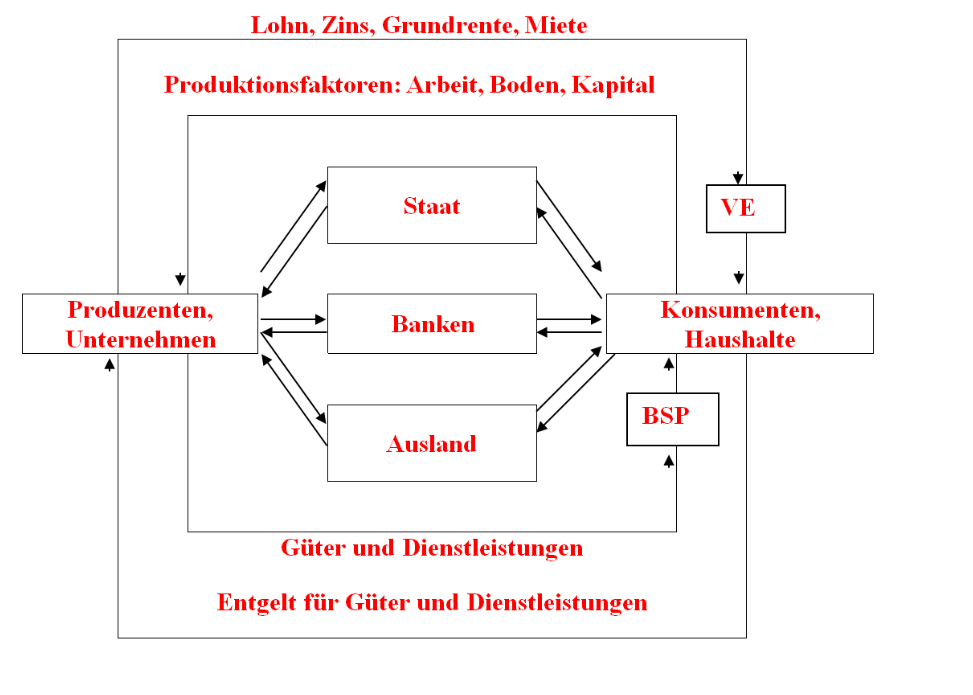
\includegraphics[keepaspectratio, width=7cm]{Wirtschaftskreislauf.png}
	\newpage
	 \begin{multicols*}{4}
	 \begin{flushleft}
	 \begin{tiny}
	 \end{tiny}
	 \end{flushleft}
	\end{multicols*}
\end{document}
